\section{Background}
\label{sec:Background}
\subsection{Tokenization}
\label{ss:tokenization}
LLMs are trained on text to predict text, and similar to other natural language processing systems, they use tokenization~\cite{webster1992tokenization} as the essential preprocessing step. It aims to parse the text into non-decomposing units called tokens. Tokens can be characters, subwords~\cite{unigramLM}, symbols~\cite{bpe}, or words, depending on the size and type of the model. Some of the commonly used tokenization schemes in LLMs are briefed here. Readers are encouraged to refer to~\cite{tokenizationsurvey} for a detailed survey.

\subsubsection{WordPiece~\cite{wordpiece}}
\label{ss:wordpiece}
It was introduced in~\cite{wordpiece} as a novel text segmentation technique for Japanese and Korean languages to improve the language model for voice search systems. WordPiece selects tokens that increase the likelihood of an n-gram-based language model trained on the vocabulary composed of tokens.

\subsubsection{BPE~\cite{bpe}}
\label{ss:bpe}
Byte Pair Encoding (BPE) has its origin in compression algorithms. It is an iterative process of generating tokens where pairs of adjacent \textit{symbols} are replaced by a new symbol, and the occurrences of the most occurring symbols in the input text are merged together.

\subsubsection{UnigramLM~\cite{unigramLM}}
\label{ss:unigramLM}
In this tokenization, a simple unigram language model (LM) is trained using an initial vocabulary of \textit{subword} units. The vocabulary is pruned iteratively by removing the lowest-probability items from the list, which are the worst performing on the unigram LM.

\subsection{Attention}
\label{ss:attention}
Attention, particularly \textit{selective attention}, has been widely studied under perception, psychophysics and psychology. Selective attention can be conceived as \enquote{the programming by the O of which stimuli will be processed or encoded and in what order this will occur}~\cite{selectiveattention}. While this definition has its roots in visual perception, it has uncanny similarities with the recently formulated \textit{attention}~\cite{attention, Transformers} (which stimuli will be processed) and \textit{positional encoding} (in what order this will occur)~\cite{Transformers} in LLMs. We discuss both in sections~\ref{ss:llmattention} and~\ref{ss:encodingposition}, respectively. 

\subsection{Attention in LLMs}
\label{ss:llmattention}
The attention mechanism computes a representation of the input sequences by relating different positions (\textit{tokens}) of these sequences. There are various approaches to calculating and implementing attention, out of which some famous types are given below.

\subsubsection{Self-Attention~\cite{Transformers}}
\label{ss:selfattention}
The self-attention is also known as intra-attention since all the queries, keys and values come from the same block (encoder or decoder). The self-attention layer connects all the sequence positions to each other with $O(1)$ space complexity which is highly desirable for learning long-range dependencies in the input. 

\subsubsection{Cross Attention}
\label{ss:crossattention}
In encoder-decoder architectures, the outputs of the encoder blocks act as the queries to the intermediate representation of the decoder, which provides the keys and values to calculate a representation of the decoder conditioned on the encoder. This attention is called cross-attention.

\subsubsection{Full Attention}
\label{ss:fullattention}
The naive implementation of calculating self-attention is known as full attention.

\subsubsection{Sparse Attention~\cite{sparse_transformer}}
\label{ss:sparseattention}
The self-attention has a time complexity of $O(n^2)$, which becomes prohibitive when scaling the LLMs to large context windows. An approximation to the self-attention was proposed in~\cite{sparse_transformer}, which greatly enhanced the capacity of GPT series LLMs to process a greater number of input tokens in a reasonable time.

\subsubsection{Flash Attention~\cite{flashattention}}
\label{ss:flashattention}
The bottleneck for calculating the attention using GPUs lies in the memory access rather than the computational speed. Flash Attention uses the classical input tiling approach in order to process the blocks of the input in GPU on-chip SRAM rather than doing IO for every token from the High Bandwith Memory (HBM). An extension of this approach to sparse attention follows the speed gains of the full attention implementation. This trick allows even greater context-length windows in the LLMs as compared to those LLMs with sparse attention.

\subsection{Encoding Positions}
\label{ss:encodingposition}
The \textit{attention} modules do not consider the order of processing by design. Transformer~\cite{Transformers} introduced \enquote{positional encodings} to feed information about the position of the tokens in input sequences. Several variants of positional encoding have been proposed~\cite{alibi, su2021roformer}. Interestingly, a recent study~\cite{NoPE} suggests that adding this information may not matter for the state-of-the-art decoder-only Transformers.

\subsubsection{Absolute}
This is the most straightforward approach to adding the sequence order information by assigning a unique identifier to each position of the sequence before passing it to the attention module.

\subsubsection{Relative}
In order to pass the information of the relative dependencies of different tokens appearing at different locations in the sequence, a relative positional encoding is calculated by some kind of learning. Two famous types of relative encodings are: 

\noindent
\emph{\textbf{Alibi}~\cite{alibi}} In this approach, a scalar bias is subtracted from the attention score calculated using two tokens which increases with the distance between the positions of the tokens. This learned approach effectively favors using recent tokens for attention. 

\noindent
\emph{\textbf{RoPE}} Keys, queries and values are all vectors in the LLMs. RoPE~\cite{su2021roformer} involves the rotation of the query and key representations at an angle proportional to their absolute positions of the tokens in the input sequence. This step results in a relative positional encoding scheme which decays with the distance between the tokens.

\subsection{Activation Functions}
\label{sec:activation functions}
The activation functions serve a crucial role in the curve-fitting abilities of the neural networks, as proved in~\cite{activationfunction}. The modern activation functions used in LLMs are different from the earlier squashing functions but are critical to the success of LLMs. We discuss these activation functions in this section.  

\subsubsection{ReLU~\cite{relu}}
\label{ss:relu}
Rectified linear unit (ReLU) is defined as
\begin{equation}
ReLU(x) = max(0,x)    
\label{eq:relu}
\end{equation}

\subsubsection{GeLU~\cite{gelu}}
\label{ss:gelu}
Gaussian Error Linear Unit (GeLU) is the combination of ReLU,  dropout~\cite{srivastava2014dropout} and zoneout~\cite{krueger2016zoneout}. It is the most widely used activation function in contemporary LLM literature.

\subsubsection{GLU variants~\cite{shazeer2020glu}}
\label{ss:gluvariants}
Gated Linear Unit~\cite{glu} is a neural network layer that is an element-wise product ($\otimes$) of a linear transformation and a sigmoid transformed ($\sigma$) linear projection of the input given as
\begin{equation}
GLU(x, W, V, b, c) = (xW + b) \otimes \sigma (xV + c),
\end{equation}
where $X$ is the input of layer and $l$, $W, b, V \textnormal{ and }c$ are learned parameters.

GLU was modified in~\cite{shazeer2020glu} to evaluate the effect of different variations in the training and testing of transformers, resulting in better empirical results. Here are the different GLU variations introduced in~\cite{shazeer2020glu} and used in LLMs. 

\begin{align*}
ReGLU(x, W, V, b, c) &= max(0, xW + b) \otimes , \\
GEGLU(x, W, V, b, c) &= GELU(xW + b) \otimes (xV + c), \\
SwiGLU(x, W, V, b, c, \beta) &= Swish\beta (xW + b) \otimes (xV + c).          
\end{align*}

\subsection{Layer Normalization}
\label{sec:layernormalization}
Layer normalization leads to faster convergence and is a widely used component in transformers. In this section, we provide different normalization techniques widely used in LLM literature.

\subsubsection{LayerNorm}
\label{ss:layernorm}
Layer norm computes statistics over all the hidden units in a layer $(l)$ as follows: 
\begin{equation}
u^l = \frac{1}{n} \sum_{i}^{n} a_i^l \hspace{2em} \sigma^l = \sqrt{\frac{1}{n} \sum_{i}^{n} (a_i^l - u^l)^2} ,
\end{equation}
where $n$ is the number of neurons in the layer $l$ and $a_i^l$ is the summed input of the $i$ neuron in layer $l$. LayerNorm provides invariance to rescaling of the weights and re-centering of the distribution.

\subsubsection{RMSNorm}
~\cite{rmsnorm} proposed that the invariance properties of LayerNorm are spurious, and we can achieve the same performance benefits as we get from LayerNorm by using a computationally efficient normalization technique that trades off re-centering invariance with speed. LayerNorm gives the normalized summed input to layer $l$ as follows
\begin{equation}
\overline{a_i^l} = \frac{a_i^l - u^l}{\sigma}g_i^l 
\end{equation}
where $g_i^l$ is the gain parameter. RMSNorm~\cite{rmsnorm} modifies $\overline{a_i^l}$ as

\begin{equation}
\overline{a_i^l} = \frac{a_i^l}{\textnormal{RMS}(\mathbf{a}^l)} g_i^l, \hspace{0.3em} \textnormal{where} \hspace{0.3em} \textnormal{RMS}(\mathbf{a}^l) = \sqrt{\frac{1}{n}\sum_{i}^{n}(a_i^l)^2}.
\end{equation}

\subsubsection{Pre-Norm and Post-Norm}
LLMs use transformer~\cite{Transformers} architecture with some variations. The original implementation~\cite{Transformers} used layer normalization after the residual connection, commonly called post-LN, concerning the order of \textit{Multihead attention – Residual – LN}. There is another order of the normalization, referred to as pre-LN~\cite{preLN} due to the position of the normalization step before the self-attention layer as in \textit{LN – Multihead attention – Residual}. Pre-LN is known to provide more stability in the training~\cite{shleifer2021normformer}. 

\subsubsection{DeepNorm}
While pre-LN has certain benefits over post-LN training, pre-LN training has an unwanted effect on the gradients~\cite{shleifer2021normformer}. The earlier layers have larger gradients than those at the bottom. DeepNorm~\cite{deepnorm} mitigates these adverse effects on the gradients. It is given as
\begin{equation}
\mathbf{x}^{l_f} = LN(\alpha \mathbf{x}^{l_p} + G^{l_p}(\mathbf{x}^{l_p}, {\boldmath\theta}{^{l_p}}), 
\end{equation}
where $\alpha$ is a constant and $\theta^{l_p}$ represents the parameters of layer $l_p$. These parameters are scaled by another constant $\beta$. Both of these constants depend only on the architecture. 

\subsection{Distributed LLM Training}
This section describes distributed LLM training approaches briefly. A more detailed discussion is available in~\cite{Survey_LLM}. 

\subsubsection{Data Parallelism}
Data parallelism replicates the model on multiple devices where data in a batch gets divided across devices. At the end of each training iteration weights are synchronized across all devices.    

\subsubsection{Tensor Parallelism}
Tensor parallelism shards a tensor computation across devices. It is also known as horizontal parallelism or intra-layer model parallelism.

\subsubsection{Pipeline Parallelism}
Pipeline parallelism shards model layers across different devices. This is also known as vertical parallelism.

\subsubsection{Model Parallelism}
A combination of tensor and pipeline parallelism is known as model parallelism.
\subsubsection{3D Parallelism}
A combination of data, tensor, and model parallelism is known as 3D parallelism.

\subsubsection{Optimizer Parallelism}
Optimizer parallelism also known as zero redundancy optimizer~\cite{ZeroOpt} implements optimizer state partitioning, gradient partitioning, and parameter partitioning across devices to reduce memory consumption while keeping the communication costs as low as possible. 

\subsubsection{Rematerialization}

\subsection{Libraries}
Some commonly used libraries for LLM training are: 1) Transformer~\cite{Lib_Transformers}, 2) DeepSpeed~\cite{Lib_DeepSpeed}, 3) Megatraon-LM~\cite{Lib_Megatron}, 4) JAX~\cite{Lib_Jax}, 5) Colossal-AI~\cite{Lib_Colossal}, 6) BMTrain~\cite{Lib_Bmtrain}, 7) FastMoE~\cite{Lib_Fastmoe}, and frameworks are 1) MindSpore~\cite{Lib_Mindspore}, 2) PyTorch~\cite{Lib_Pytorch}, 3) Tensorflow~\cite{Lib_Tensorflow}, 4) MXNet~\cite{Lib_Mxnet}.  

\subsection{Data PreProcessing}
This section briefly summarizes data preprocessing techniques used in LLMs training. More details on this are available in~\cite{Survey_LLM}.

\subsubsection{Quality Filtering}
For better results, training data quality is essential. Some approaches to filtering data are: 1) classifier-based and 2) heuristics-based. Classifier-based approaches train a classifier on high-quality data and predict the quality of text for filtering, whereas heuristics-based employ some rules for filtering like language, metrics, statistics, and keywords. 

\subsubsection{Data Deduplication}
Duplicated data can affect model performance and increase data memorization; therefore, to train LLMs, data deduplication is one of the preprocessing steps. This can be performed at multiple levels, like sentences, documents, and datasets.

\subsubsection{Privacy Reduction}
Most of the training data for LLMs is collected through web sources. This data contains private information; therefore, many LLMs employ heuristics-based methods to filter information such as names, addresses, and phone numbers to avoid learning the mentioned information.

\subsection{Architectures}
Here we discuss the variants of the transformer architectures at a higher level which arise due to the difference in the application of the attention and the connection of transformer blocks. An illustration of attention patterns of these architectures is shown in Figure~\ref{architectures}.

\subsubsection{Encoder Decoder}
Transformers were originally designed as sequence transduction models and followed other prevalent model architectures for machine translation systems. They selected encoder-decoder architecture to train human language translation tasks. This architecture is adopted by~\cite{T5, UL2}. In this architectural scheme, an encoder encodes the input sequences to variable length context vectors, which are then passed to the decoder to maximize a joint objective of minimizing the gap between predicted token labels and the actual target token labels.

\subsubsection{Causal Decoder}
The underlying objective of an LLM is to predict the next token based on the input sequence. While additional information from the encoder binds the prediction strongly to the context, it is found in practice that the LLMs can learn as well absent this encoder~\cite{decoderonly} and adding the context in the decoder. Similar to the original encoder-decoder architecture's decoder block, this decoder restricts the flow of information backward, i.e., the predicted token $t_k$ only depends on the tokens preceded by and up to $t_{k-1}$. This is the most widely used variant in the state-of-the-art LLMs.

\subsubsection{Prefix Decoder}
The causal masked attention is reasonable in the encoder-decoder architectures where the encoder can attend to all the tokens in the sentence from every position using self-attention. This means that the encoder can also attend to tokens $t_{k+1}$ to $t_n$ in addition to the tokens from $t_1$ to $t_{k-1}$ while calculating the representation for $t_k$. But when we drop the encoder and only keep the decoder, we also lose this flexibility in attention. A variation in the decoder-only architectures is by changing the mask from strictly causal to fully visible on a portion of the input sequence, as shown in Figure~\ref{architectures}. The Prefix decoder is also known as non-causal decoder architecture.

%\subsubsection{Mixture of Experts}
%\SA{Check this?}
% We will discuss this in next version

\begin{figure}[tbp]
\centering
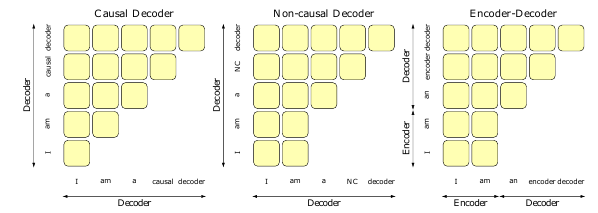
\includegraphics[width=1\columnwidth]{Figure/architectures.png}
\caption{An example of attention patterns in language models, image is taken from~\cite{LLM_Objectives}.}
\label{architectures}
\end{figure}

\subsection{Pre-Training Objectives}
\label{sec:pretrainobjectives}
This section describes LLMs pre-training objectives. For more details see the paper~\cite{LLM_Objectives}. 

\subsubsection{Full Language Modeling}
An autoregressive language modeling objective where the model is asked to predict future tokens given the previous tokens, an example is shown in Figure~\ref{t_objectives}. 

\subsubsection{Prefix Language Modeling}
A non-causal training objective, where a prefix is chosen randomly and only remaining target tokens are used to calculate the loss. An example is shown in Figure~\ref{t_objectives}.

\subsubsection{Masked Language Modeling}
In this training objective, tokens or spans (a sequence of tokens) are masked randomly and the model is asked to predict masked tokens given the past and future context. An example is shown in Figure~\ref{t_objectives}. 

\subsubsection{Unified Language Modeling}
Unified language modeling~\cite{Unified_LM} is a combination of causal, non-causal, and masked language training objectives. Here in masked language modeling, the attention is not bidirectional but unidirectional, attending either left-to-right or right-to-left context.
\begin{figure}[tbp]
\centering
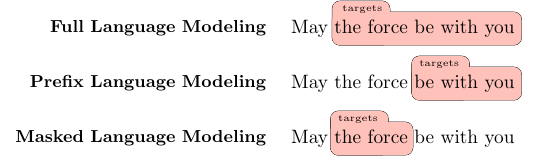
\includegraphics[width=1\columnwidth]{Figure/training_objectives.png}
\caption{An example of language model training objectives, image from~\cite{LLM_Objectives}.}
\label{t_objectives}
\end{figure}

\subsection{Model Adaptation}
This section discusses various model adaptation techniques, where a model is pre-trained on large data and then adapted for downstream tasks. 

\subsubsection{Transfer Learning}
Fine-tuning a pre-trained model with data for the downstream task is known as transfer learning. In this type of model adaptation, the model is initialized with pre-trained weights and updated according to the new data. Some of the LLMs employing this technique are~\cite{T5, mT5, UL2, U-PaLM}. 

\subsubsection{Parameter Efficient Learning}
The parameter efficient learning fine-tunes a few parameters either by adding new parameters to the model or the existing ones. 

\vspace{1mm}
\noindent
\emph{\textbf{Prompt Tuning:}}~\cite{Prompt_Tuning, Prompt_Tuning_2} adds trainable prompt token embeddings as prefixes or free-style to the input token embeddings. During fine-tuning only these embeddings parameters are trained for the downstream task while keeping the rest of the weights frozen.

\vspace{1mm}
\noindent
\emph{\textbf{Prefix Tuning:}}~\cite{Prefix_Tuning} adds task-specific trainable prefix vectors to the transformer layers, where only prefix parameters are fine-tuned, and the rest of the model stays frozen. The input sequence tokens can attend prefixes acting as virtual tokens.    

\vspace{1mm}
\noindent
\emph{\textbf{Adapter Tuning:}} module is an encoder-decoder architecture that is placed either sequential or parallel to the attention and feed-forward layers in the transformer block~\cite{LMAdapter, LMAdapter_2, LMAdapter_3}. Only these layers are fine-tuned, and the rest of the model is kept frozen.  

\subsubsection{Instruction Finetuning}
Instruction tuning is an approach to fine-tuning pre-trained models on instruction formatted data. Instructions generally comprise multiple tasks in plain natural language, guiding the model to respond according to the prompt and the input. The training data consists of an instruction and an input-output pair. More details on formatting instruction data and its various styles are available in~\cite{Survey_LLM}.     

\subsubsection{Alignment Tuning}
LLMs are prone to generate false, biased, and harmful text. Therefore, models are aligned using human feedback to make them helpful, honest, and harmless. Alignment involves asking LLMs to generate unexpected responses and then updating their parameters to avoid such responses~\cite{Survey_LLM}.

\subsubsection{In-context Learning} 
No fine-tuning is involved in this type of model adaptation. The model is shown multiple input-output demonstration pairs to generate a desired input response. This adaptation is similar to a few-shot learning but without requiring any parameter update. More details on formatting demonstrations are available in~\cite{Survey_LLM}. 
 
\subsubsection{Chain-of-thought Prompting}
Chain-of-thought prompting (CoT) is a special case of prompting where demonstrations contain reasoning information aggregated with inputs and outputs so that the model generates outcomes with reasonings. Some examples in literature train LLMs with CoT reasoning, whereas other utilizes LLMs' CoT abilities without fine-tuning. More details on designing prompts are available in~\cite{Survey_LLM}.

